\documentclass[cn,10pt,math=newtx,color=blue]{elegantbook}
\usepackage{fontspec}
\setmonofont{Consolas}
% \usepackage{amsmath}
\usepackage{graphicx}
\usepackage[a4paper,scale=0.8,centering]{geometry}
\usepackage{caption,subcaption}
\usepackage{tcolorbox}
\usepackage[colorlinks=true]{hyperref}
\tcbuselibrary{most}
%\newenvironment{myquotaion}{\begin{quotation}}{\end{quotation}}
%\tcolorboxenvironment{myquotaion}
%{enhanced, breakable,colback = white, colframe = cyan, colbacktitle = cyan, attach boxed title to top left = {yshift = -2mm, xshift = 5mm},boxed title style = {sharp corners},fonttitle = \sffamily\bfseries}
\newtcolorbox{myquotation}[1]{enhanced, breakable,colback = white, colframe = cyan, colbacktitle = cyan, attach boxed title to top left = {yshift = -2mm, xshift = 5mm},boxed title style = {sharp corners},fonttitle = \bfseries,title={#1}}

%\usepackage{pythonhighlight}
\usepackage{minted}
\usepackage{listings}
% 用来设置附录中代码的样式
% \lstset{
%     basicstyle          =   \ttfamily,          % 基本代码风格
%     keywordstyle        =   \bfseries,          % 关键字风格
%     commentstyle        =   \rmfamily\itshape,  % 注释的风格,斜体
%     stringstyle         =   \ttfamily,  % 字符串风格
%     flexiblecolumns,                % 别问为什么,加上这个
%     numbers             =   left,   % 行号的位置在左边
%     showspaces          =   false,  % 是否显示空格,显示了有点乱,所以不现实了
%     numberstyle         =   \zihao{-5}\ttfamily,    % 行号的样式,小五号,tt等宽字体
%     showstringspaces    =   false,
%     captionpos          =   t,      % 这段代码的名字所呈现的位置,t指的是top上面
%     frame               =   lrtb,   % 显示边框
% }

\definecolor{mGreen}{rgb}{0,0.6,0}
\definecolor{mGray}{rgb}{0.5,0.5,0.5}
\definecolor{mPurple}{rgb}{0.58,0,0.82}
\definecolor{backgroundColour}{rgb}{0.95,0.95,0.92}

\lstset{
    basicstyle=\ttfamily,
    backgroundcolor=\color{backgroundColour},
    keywordstyle=\color{purple}\bfseries,
    % identifierstyle=\color{brown!80!black},
    commentstyle=\color{gray}
    showstringspaces=false,
}

\lstdefinestyle{Python}{
    language        =   Python, % 语言选Python
    basicstyle      =   \zihao{-5}\ttfamily,
    numberstyle     =   \zihao{-5}\ttfamily,
    keywordstyle    =   \color{blue},
    keywordstyle    =   [2] \color{teal},
    stringstyle     =   \color{magenta},
    commentstyle    =   \color{red}\ttfamily,
    breaklines      =   true,   % 自动换行,建议不要写太长的行
    columns         =   fixed,  % 如果不加这一句,字间距就不固定,很丑,必须加
    basewidth       =   0.5em,
}



\lstdefinelanguage{CAPL}
{
    morekeywords={byte, dword, }, %定义关键字
    sensitive=false, %是否大小写敏感
}

\lstdefinestyle{C}{
    backgroundcolor=\color{backgroundColour},   
    commentstyle=\color{mGreen},
    % keywordstyle=\color{magenta},
    numberstyle=\tiny\color{mGray},
    stringstyle=\color{mPurple},
    basicstyle=\footnotesize\ttfamily,
    breakatwhitespace=false,         
    breaklines=true,                 
    captionpos=b,                    
    keepspaces=true,                 
    numbers=left,                    
    numbersep=5pt,                  
    showspaces=false,                
    showtabs=false,                  
    tabsize=4,
    language=C
}

\usepackage{hyperref}
\newcommand{\tabincell}[2]{\begin{tabular}{@{}#1@{}}#2\end{tabular}}
\title{学习笔记}
% \subtitle{Elegant\LaTeX{} 经典之作}

\author{Wang Haojiang}
% \institute{Elegant\LaTeX{} Program}
\date{Dec 1, 2021}
\version{1.0}
\bioinfo{自定义}{信息}

% \extrainfo{各人自扫门前雪,休管他人瓦上霜。—— 陈元靓}

\setcounter{tocdepth}{3}

\logo{logo-blue.png}
\cover{cover.jpg}
\definecolor{customcolor}{RGB}{32,178,170}
\colorlet{coverlinecolor}{customcolor}

\begin{document}
	\maketitle
	\frontmatter
	\tableofcontents
	\mainmatter
	\chapter{MCAL配置}
\section{CAN}
% \input{ch1/section2}
% \input{ch1/section3}
% \input{ch1/section4}
% \input{ch1/section5}
% \input{ch1/section6}
% \input{ch1/section7}
% \input{ch1/section8}
	\chapter{以太网配置}
\section{CAN}
\section{CANoe 以太网工程配置}
本节基于vector vn5620 硬件,对 CANoe 软件中以太网相关的配置方法进行总结。

\subsection{工程配置---Network-based Access}
硬件设备从固件版本 11.1 后,支持新的以太网配置方式,称为 Network-based Access。新固件下支持以下功能:

\begin{itemize}
    \item 网络和端口定义
    \item 自由的设备分片
    \item 以太网接口-PC 连接
    \item 硬件过滤
\end{itemize}
\subsubsection{基础概念}
新的模式下,存在以下几个概念,详细模块如图所示:

\begin{figure}[ht]
    \centering
    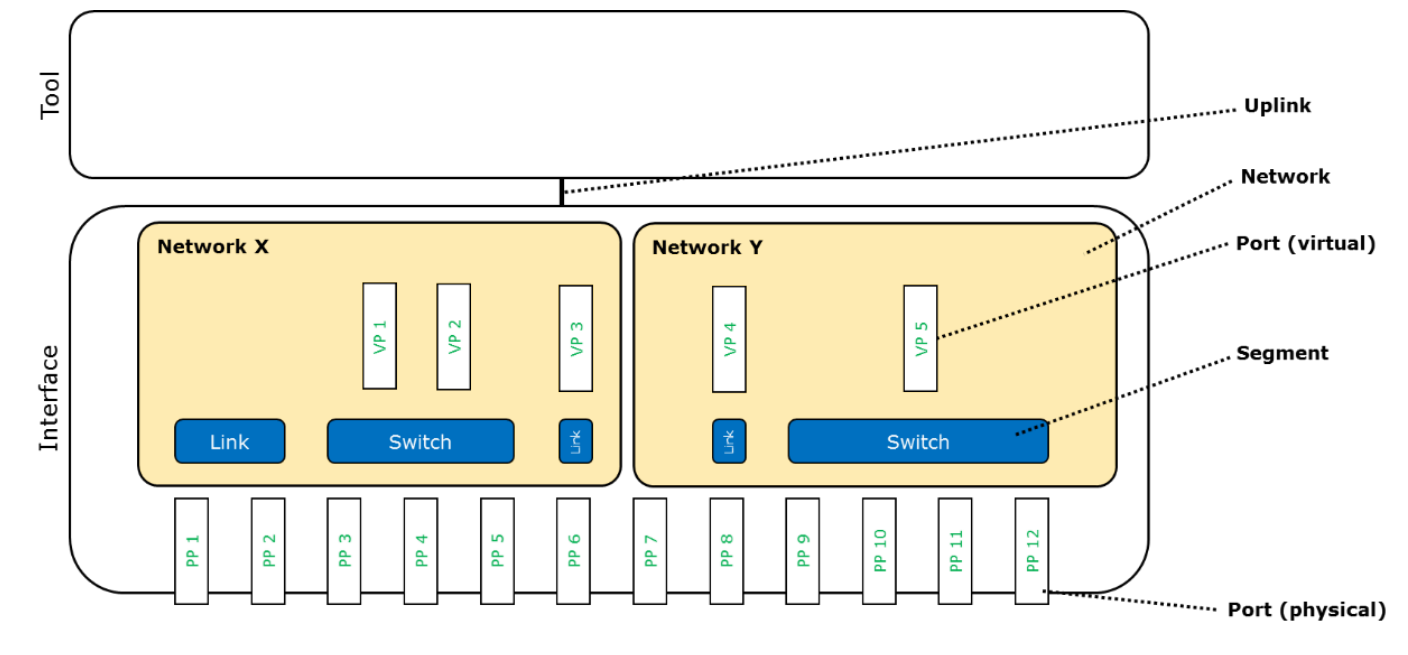
\includegraphics[scale=0.7]{pic/Snipaste_2021-10-29_09-46-43.png}
    \caption{术语实例}
    \label{fig:new_terms}
\end{figure}

\begin{enumerate}
    \item Port: 软件或硬件接入设备的入口,所以也分为物理端口和虚拟端口。CANoe 中仿真节点接入的就是虚拟端口。一个端口只能被一个 segment 包含。
    \item Segment: 分片是端口的组合。 必须至少创建一个分片并连接到一个物理端口。 每个分片都有一个唯一的名称,并且恰好分配给一个网络。 有两种类型的段可用:switch 和 link。 
    \begin{enumerate}
        \item switch segment: 提供 2 层交换机的功能。
        \item link segment: 完全透明地连接两个端口。 用于透明地转发以太网数据包和物理层的状态。Link segment 存在两种连接方式:TAP 和 直连。TAP 模式下,两个物理端口间有很小的延迟($\leq 6 \mu s$)。类似之前固件中提供的 MAC 旁路功能。
        直连模式适用于一个物理端口和虚拟端口间的连接。
    \end{enumerate}

    \item Network: 一个网络包括一个或多个分片。硬件设备中至少需要定义一个网络。
    \item Uplink: 设备和 CANoe PC 间的连接称为 uplink,可以通过配置 filter 减少传输给上位机的数据量。
\end{enumerate}

\subsubsection{概念变更}

\begin{figure}[ht]
    \centering
    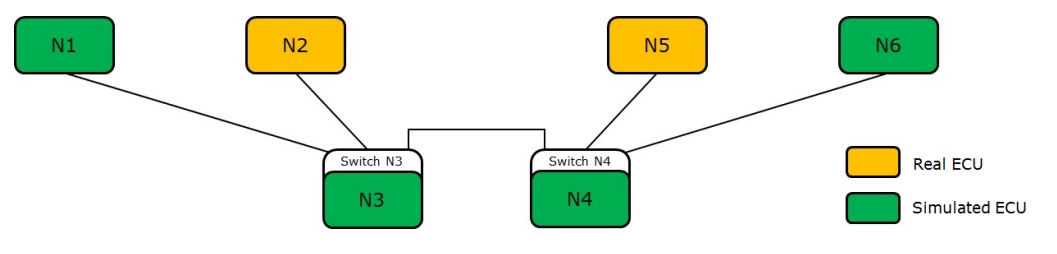
\includegraphics[scale=0.7]{pic/Snipaste_2021-10-29_14-37-48.png}
    \caption{拓扑实例}
    \label{fig:example_topology}
\end{figure}
图\ref{fig:example_topology} 包含两个复杂网络节点 \textbf{N3} 和 \textbf{N4},各自集成了一个 switch。
另外每个 switch 上连接了一个仿真节点 \textbf{N1} 和  \textbf{N6}。两个真实节点  \textbf{N2} 和  \textbf{N5}。

下图 \ref{fig:two_setup} 展示了固件版本 11.1 前后的实现方法。

\begin{figure}[ht]
    \centering
    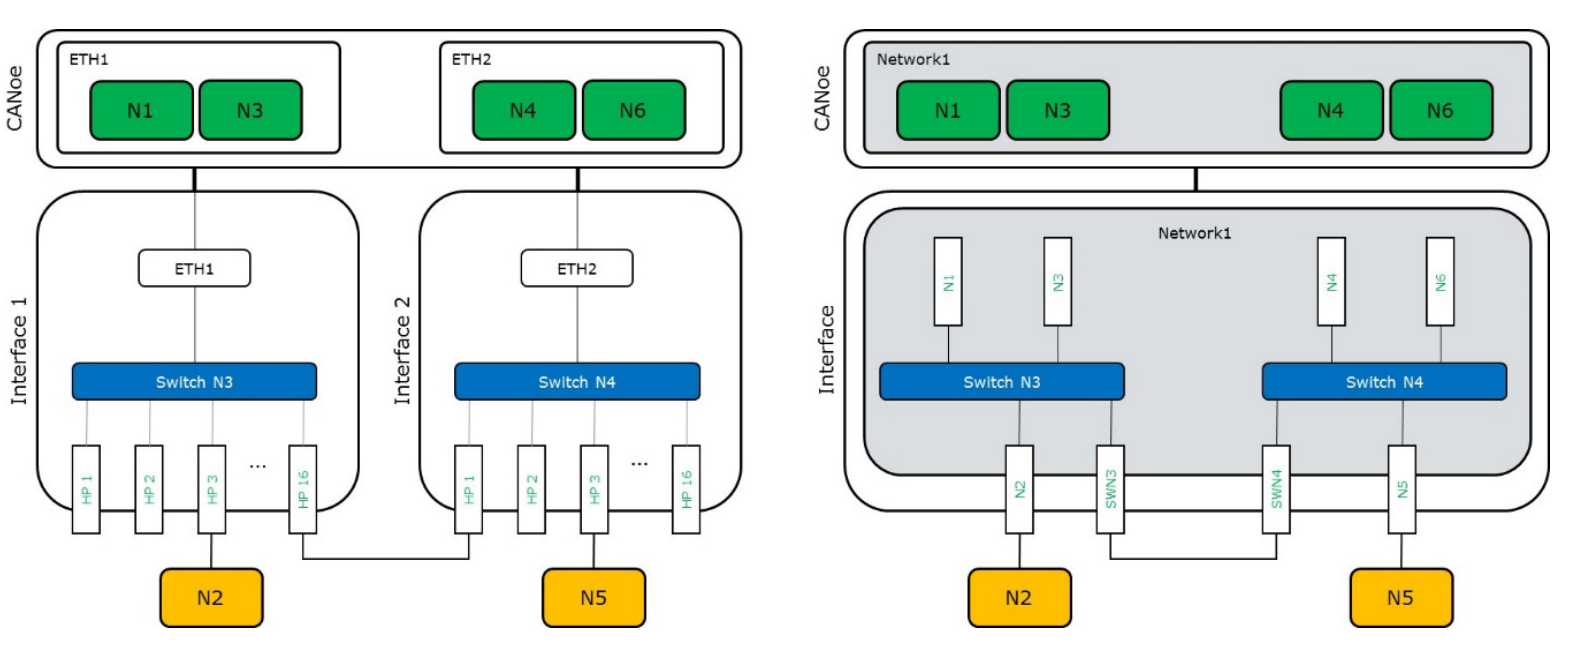
\includegraphics[scale=0.6]{pic/Snipaste_2021-10-29_14-42-44.png}
    \caption{ Simulation setup of the device firmware before version 11.1 vs. simulation setup of the device firmware from version 11.1}
    \label{fig:two_setup}
\end{figure}

之前版本中,一个设备仅能配置一个 switch 分片,因此,需要两个设备通过两个通道接入 CANoe。所以,在 CANoe 中需要配置两个 network。
之后版本中,允许自由配置分片。因此,可以配置两个 switch 分片,两个分片都分配在一个 network 中。因此,在 CANoe 中,仅需要配置一个 network。

\subsubsection{以太网包的收发方向}
设备接口接收到的以太网数据包总是标有 Rx 方向。 在这种情况下,数据包是由应用程序(例如 CANoe 模拟节点)生成还是来自真实网络无关紧要。
从接口发送到真实网络或模拟节点的数据包(例如,由于交换机段中的转发规则)被标记为 Tx 数据包。 
\begin{note}
    简单理解,新的方向,就是以硬件设备自身的角度考虑。从真实节点或仿真节点发给设备的都是 Rx 数据包,从设备发出去的都是 Tx 数据包。
\end{note}

\subsubsection{以太网硬件配置}
以太网硬件接口配置在 \textbf{Vector Hardware Config} 窗口中。如下图所示。
可以打开 \textbf{Ethernet Device Configuration}。

\begin{figure}[ht]
    \centering
    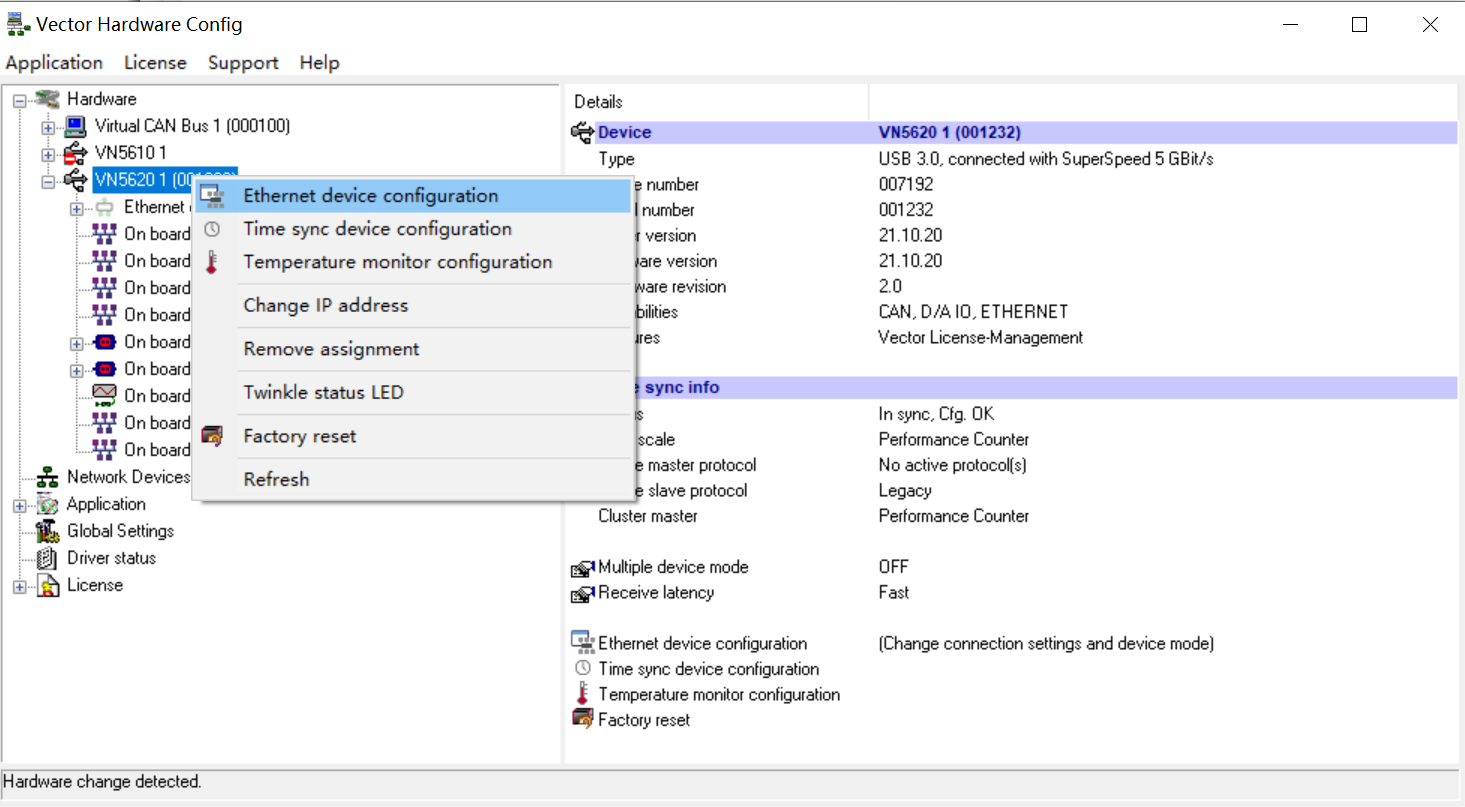
\includegraphics[scale=0.6]{pic/Snipaste_2021-10-29_15-00-01.png}
    \caption{ \textbf{Ethernet Device Configuration} 配置界面}
    \label{fig:Ethernet_Device_Configuration}
\end{figure}

下图\ref{fig:three_connect_ways}展示了三种连接方式,分别为:
\begin{itemize}
    \item 真实节点和仿真节点通过 switch 连接
    \item 真实节点和仿真节点直连
    \item 两个真实节点旁路连接,CANoe 作为检测
\end{itemize}

\begin{figure}[!ht]
    \centering
    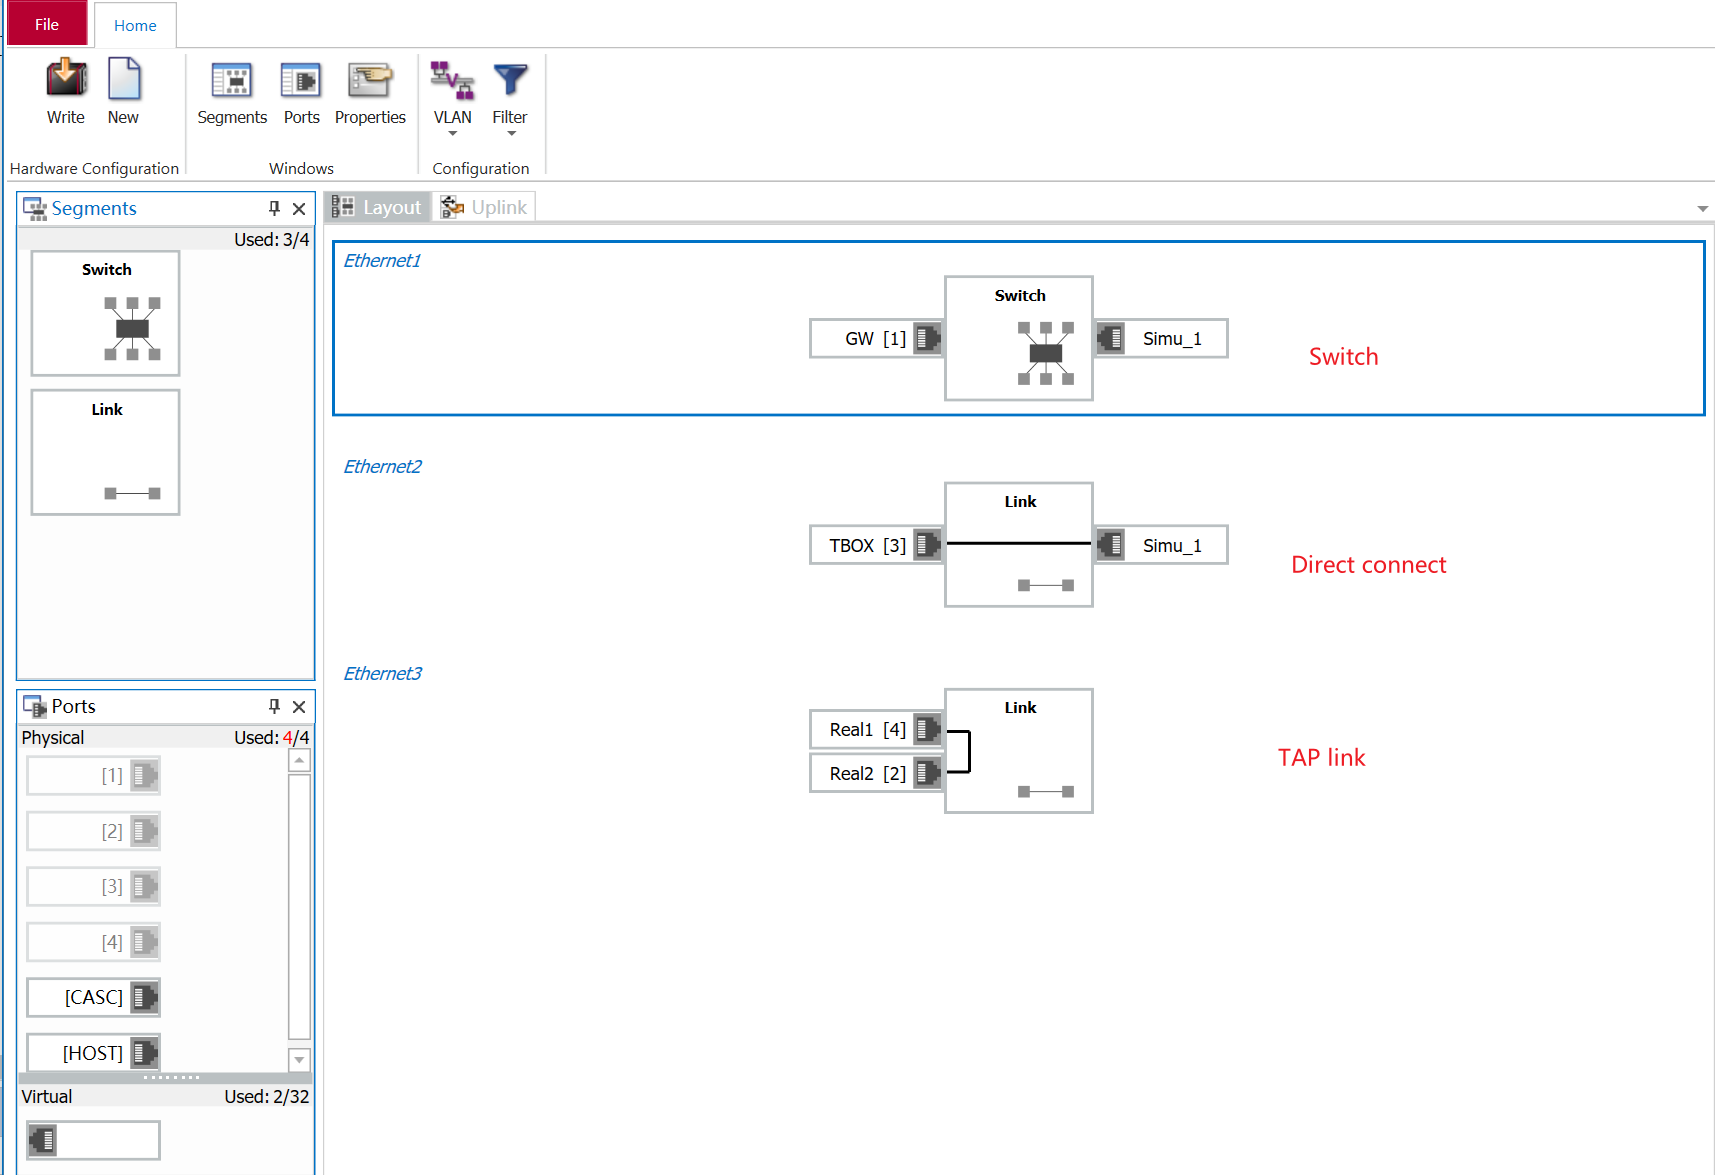
\includegraphics[scale=0.5]{pic/Snipaste_2021-10-29_15-06-06.png}
    \caption{三种连接方式}
    \label{fig:three_connect_ways}
\end{figure}

以第三种 TAP 连接方式为例,完成以上配置后,需要对以太网使用通道、通道和 network 映射、端口等进行详细配置。通道使用配置见下图\ref{fig:eth_channel_usage} \footnote{在实际使用中,仅需要使能 1 个通道,否则会报通道分配错误,详见图\ref{fig:eth_channel_usage_error}}。

\begin{figure}[ht]
    \centering
    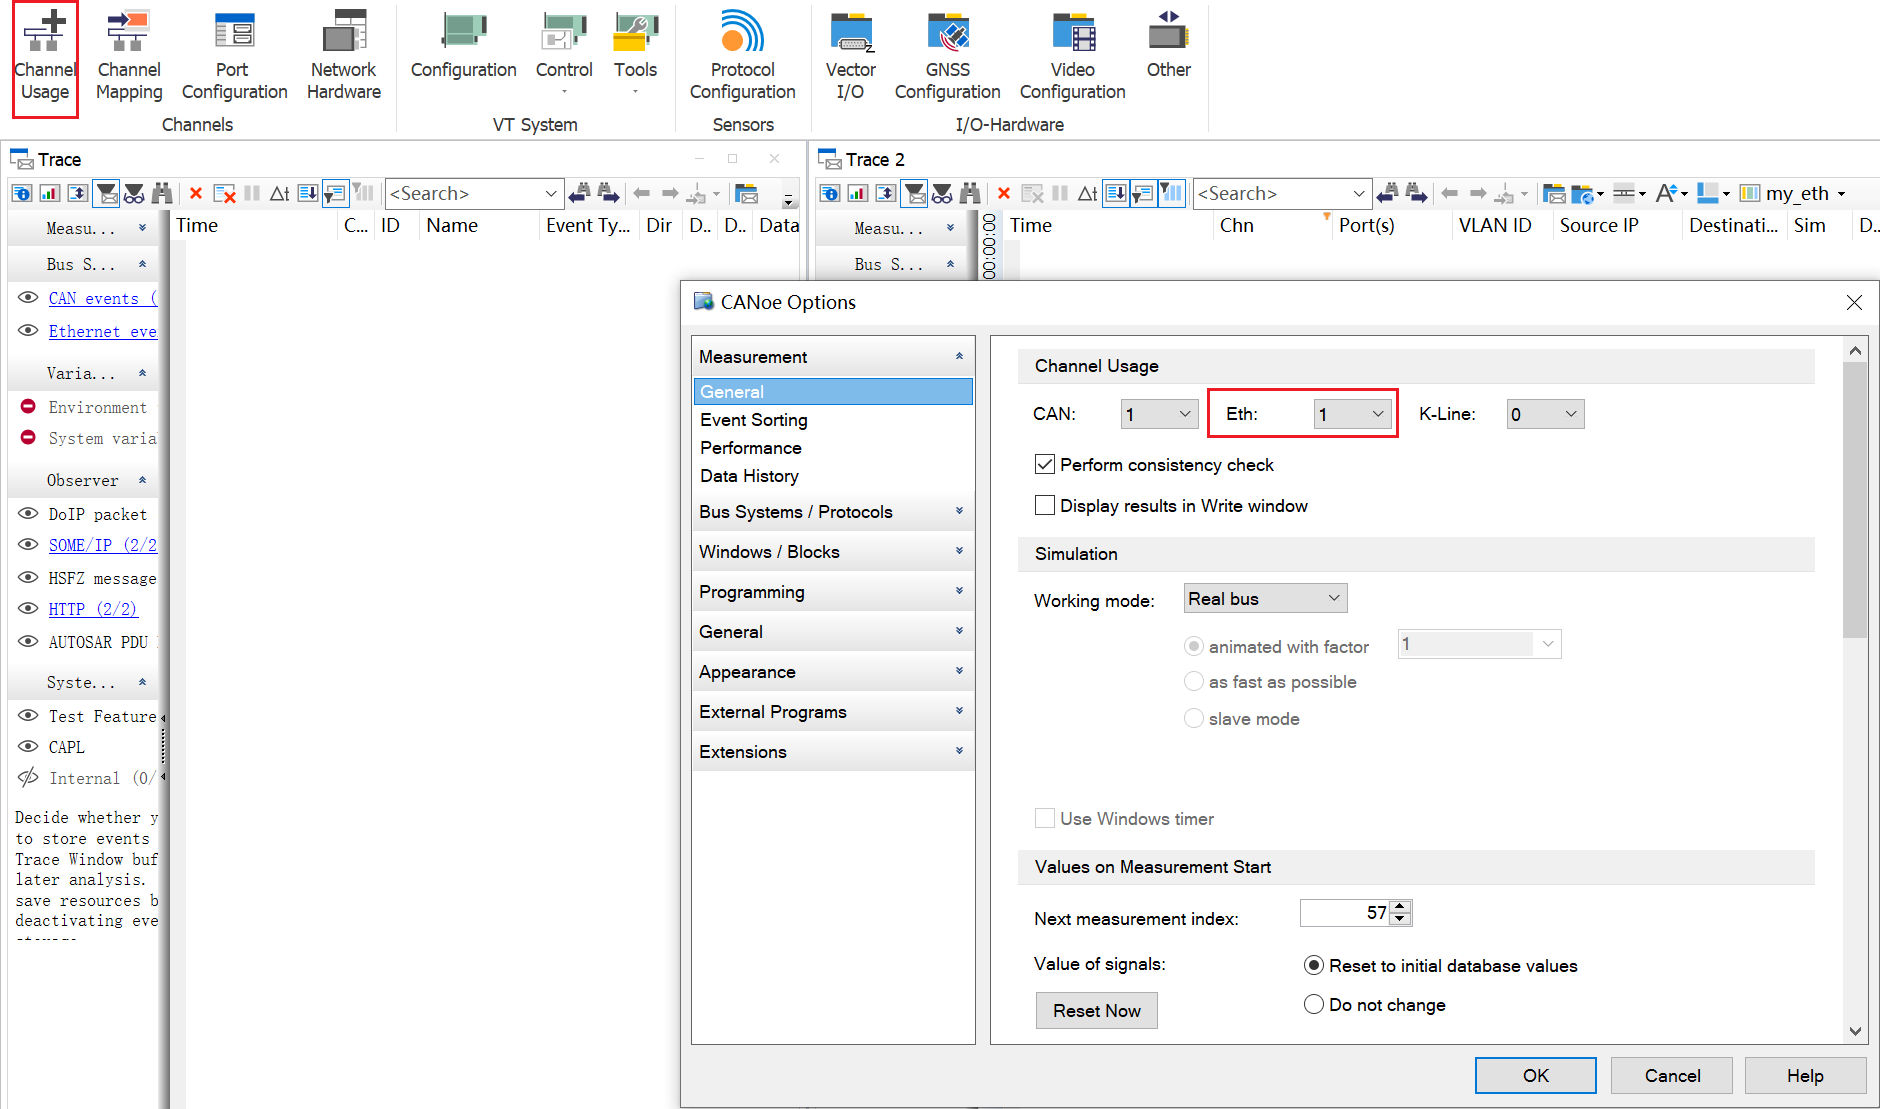
\includegraphics[scale=0.5]{pic/Snipaste_2021-10-29_15-18-52.png}
    \caption{以太网通道使用配置}
    \label{fig:eth_channel_usage}
\end{figure}

\begin{figure}[!ht]
    \centering
    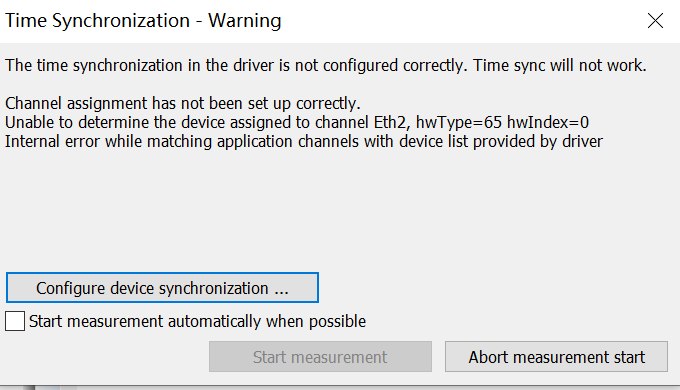
\includegraphics[scale=1]{pic/Snipaste_2021-10-29_15-22-58.png}
    \caption{以太网通道配置错误}
    \label{fig:eth_channel_usage_error}
\end{figure}

以太网通道映射,需要将以太网通道和 Simulation Setup 中定义的 Network 及 实际硬件配置的 network进行映射。详见图\ref{fig:eth_channel_mapping}。
\begin{figure}[!ht]
    \centering
    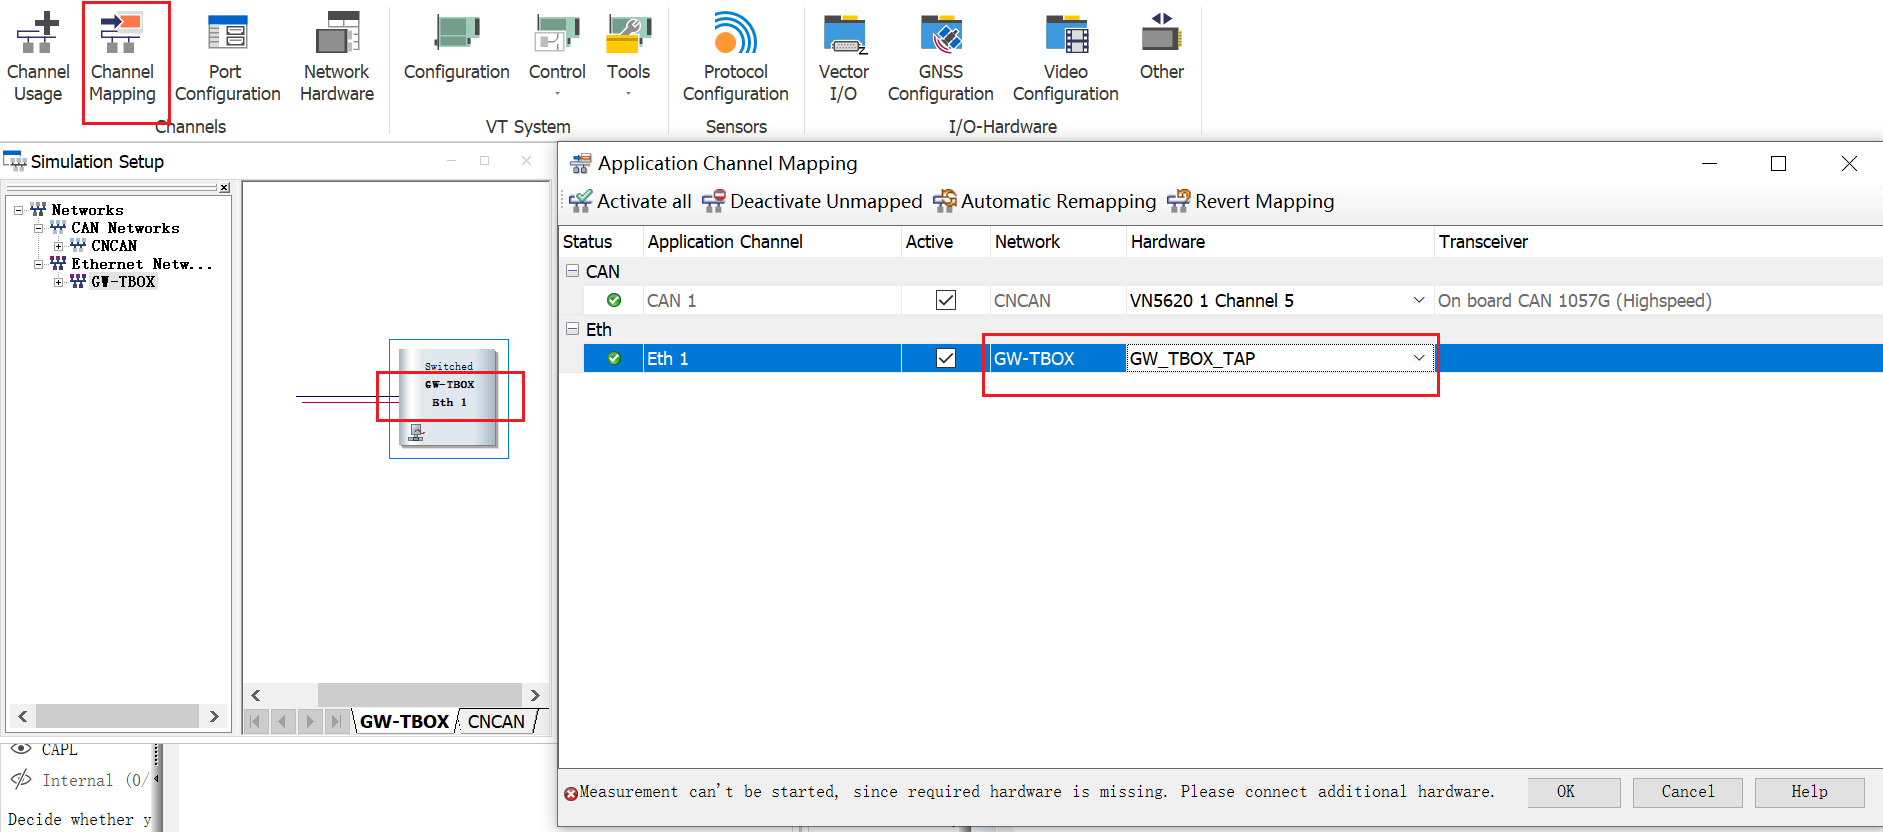
\includegraphics[scale=0.5]{pic/Snipaste_2021-10-29_15-25-55.png}
    \caption{以太网通道映射}
    \label{fig:eth_channel_mapping}
\end{figure}

最后,需要对端口状态进行配置,如进行激活等。详见图\ref{fig:port_Configuration}。
\begin{figure}[!ht]
    \centering
    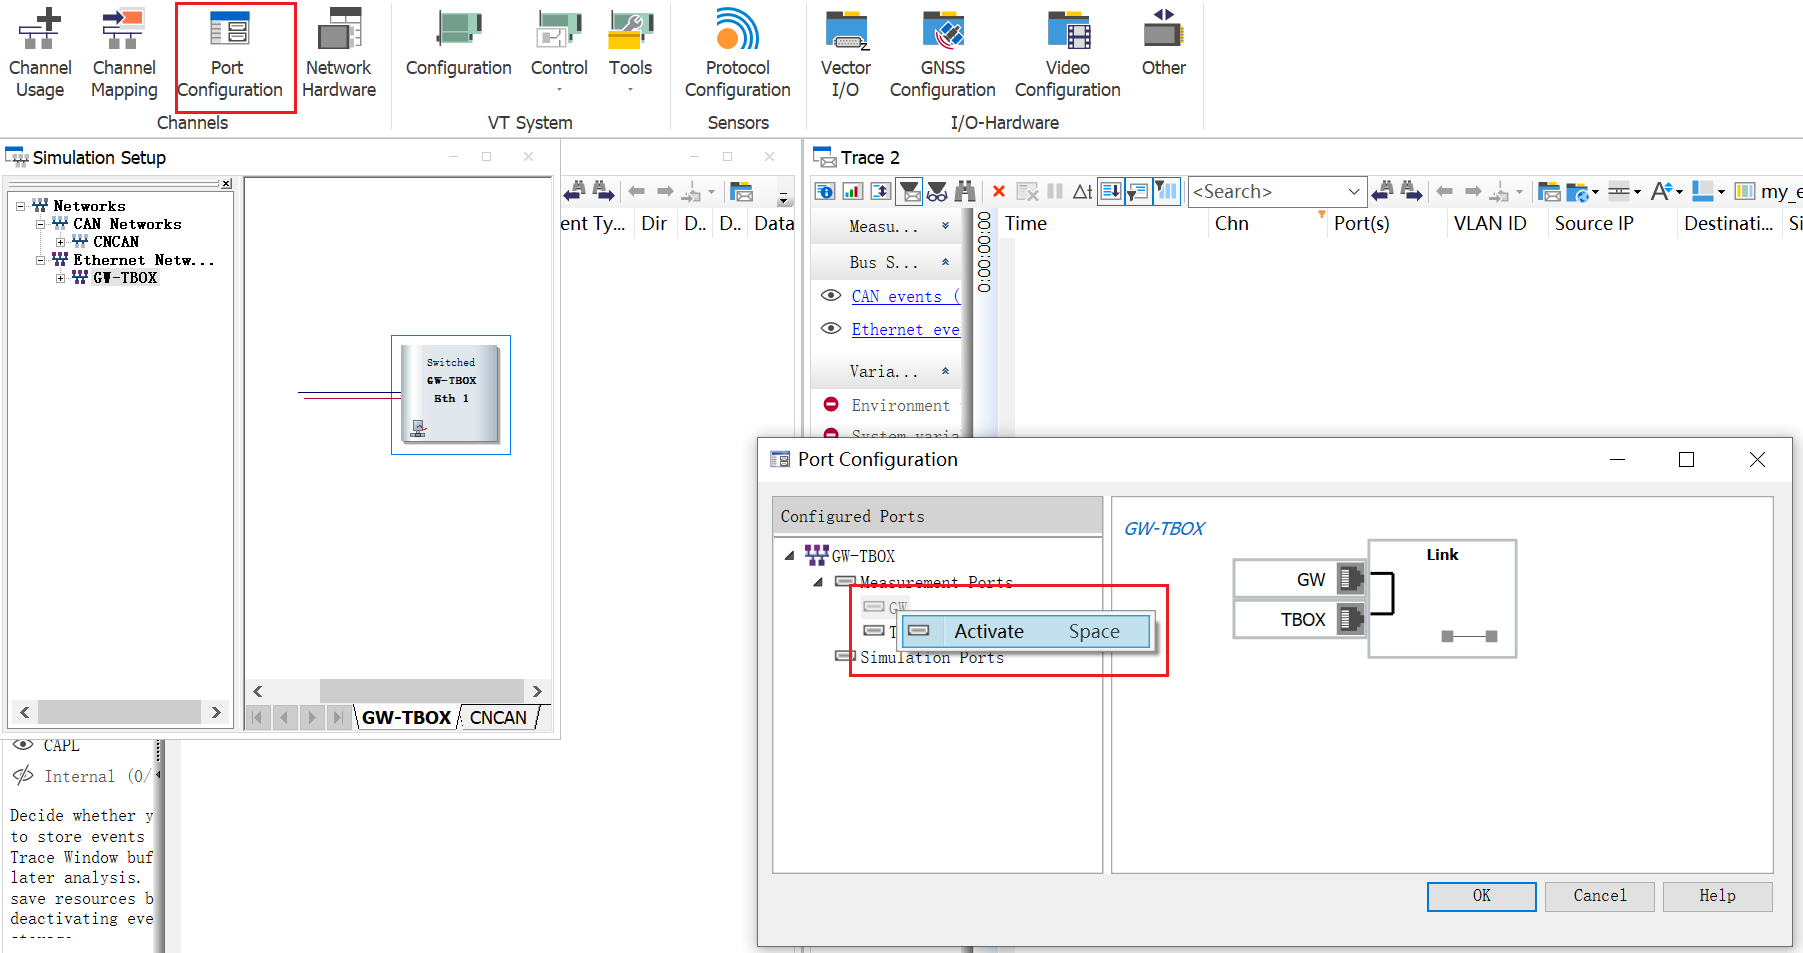
\includegraphics[scale=0.5]{pic/Snipaste_2021-10-29_15-29-21.png}
    \caption{以太网端口配置}
    \label{fig:port_Configuration}
\end{figure}

\subsection{TcpIp 协议栈配置}\label{sec:two_node_comm}
协议栈配置步骤中,主要对TCP/IP协议栈中的IP地址,mac 地址,VLAN 等配置。
以一个真实节点 GW 和一个仿真节点 ECU1 的通信为例,两节点通过 Link Direct 连接。对 ECU1 协议栈的配置如图\ref{fig:tcpip_Configuration}所示。

\begin{figure}[!ht]
    \centering
    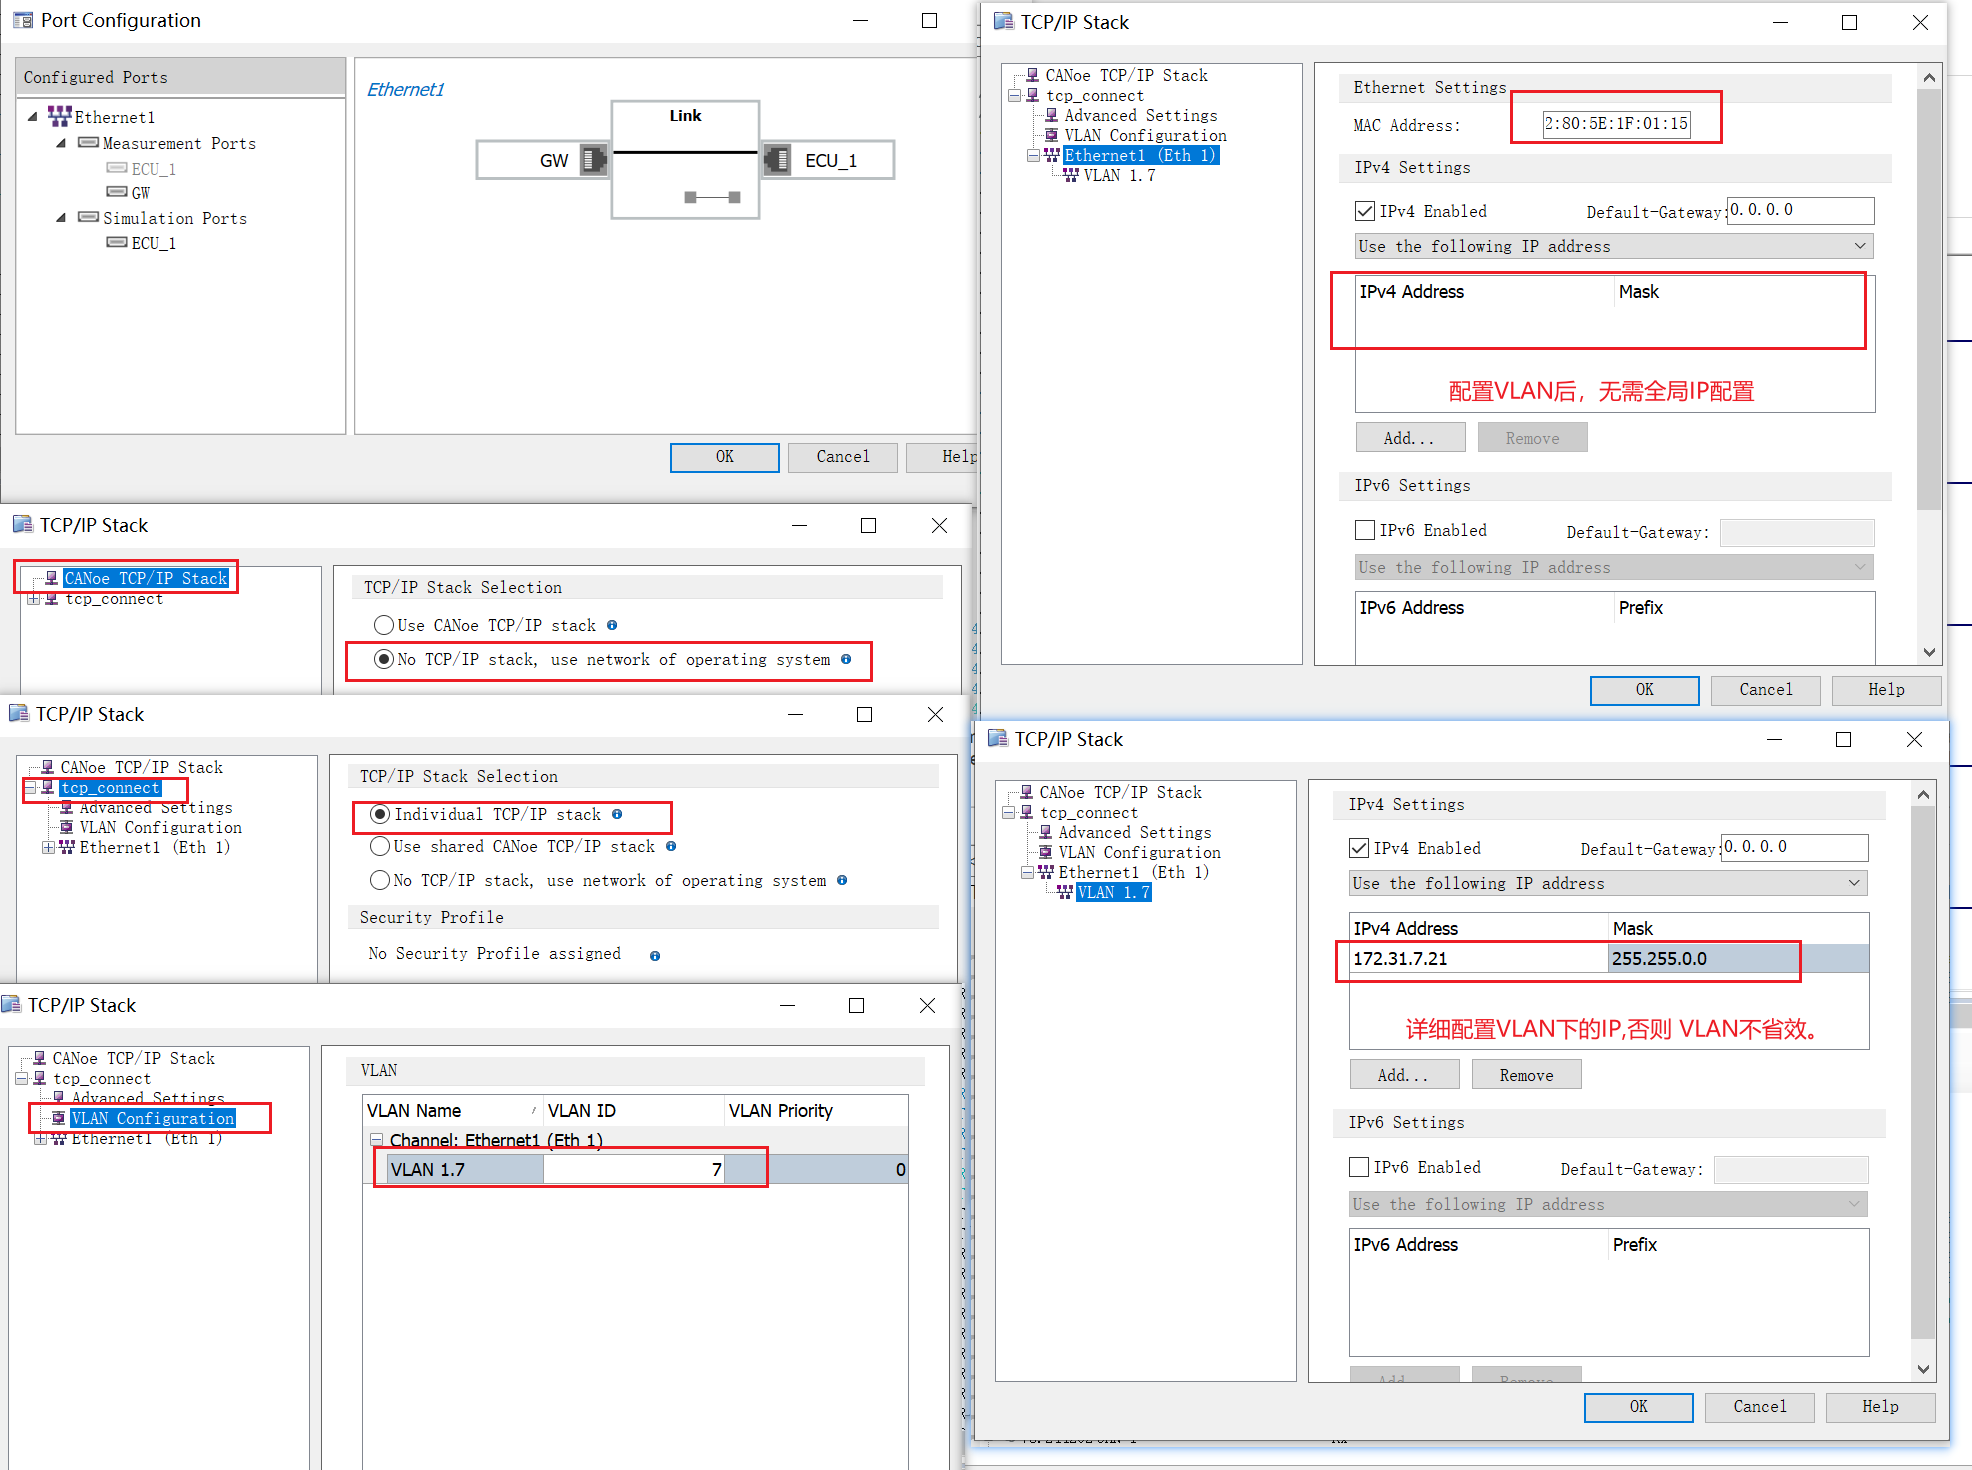
\includegraphics[scale=0.5]{pic/Snipaste_2021-10-29_16-08-23.png}
    \caption{以太网协议栈配置}
    \label{fig:tcpip_Configuration}
\end{figure}

\begin{note}
    当需要配置 VLAN 时,仿真节点协议栈中,一定要在 VLAN 详细配置中,添加对应的IP地址,否则,不能正常收发带正确 VLAN tag 的以太网帧,导致仿真结果出错。
\end{note}

\subsection{CAPL 仿真以太网节点}
以第\ref{sec:two_node_comm}节一个真实节点和一个仿真节点的通信为例,仿真节点的 CAPL 代码实现如下。
实现功能为:

\begin{enumerate}
    \item 启动后,发出 0x401 帧唤醒网络,并同时发出 0x459 帧,激活以太网DoIP功能。
    \item 等待 10s后,发起 TCP 握手,建立 TCP 连接。
    \item 等待 20s后,停发唤醒信号和以太网激活信号。
    \item 等待 60s后,网络应当休眠,重启计数器,循环上述过程。
\end{enumerate}

\lstinputlisting[
    style       =   C,
    % language = CAPL,
    language = C,
    caption     =   {仿真代码示例},
    % label       =   {ff.py}
]{ch2/gw_tbox_simu.c}

\chapter{Switch 使用}
\section{Swtich 基本功能描述}


Marvell 88Q5050 是一款具有 8 路端口的交换机芯片,在汽车领域广泛应用。可以配置支持 IEEE 100BASE-T1,100BASE-TX,RGMI/RMII/MII,GMII 和 SGMII 端口。该芯片将低功耗的 Phy 芯片和 MAC 
集成到内部,可满足 IEEE 802.3 标准。IEEE 100BASE-T1 Phy 可满足 OPEN Aliance BroadR-Reach。

\subsection{支持接口}
88Q5050 可支持接口如下:
\begin{itemize}
    \item 4 x IEEE 100BASE-T1 (IEEE 802.3bw)
    \item 额外 6 路可配置端口(同时可打开 4 路)
    \begin{itemize}
        \item 1 x IEEE 100BASE-T1
        \item 1 x IEEE 100BASE-TX
        \item 2 x MII/RMII/RGMII
        \item 1 x MII
        \item 1 x MII
        \item 1 x SGMII 
    \end{itemize}
    \item 2 x SMI
    \item 可配置 GPIO
    \item QSPI 可配置频率 19.2 ~ 83.3 MHz
    \item EEPROM 从接口,可配置E2大小 32 ~ 512 Kb
\end{itemize}

表\ref{tab:port_interface}汇总了芯片接口类型,每一行代表了一种组合。

% Table generated by Excel2LaTeX from sheet 'Sheet1'
\begin{table}[htbp]
    \centering
    
    \caption{Port 接口汇总}
      \begin{tabular}{lllllr}
      \toprule
      Ports 1 to 4 & Port 5 & Port 6 & Port 7 & Port 8 & Notes \\
      \midrule
      100BASE-T1 & 100BASE-T1 & 100BASE-TX & SGMII & xMII  &  \\
      \tabincell{l}{100BASE-T1} & \tabincell{l}{xMII}  & \tabincell{l}{100BASE-TX} & \tabincell{l}{SGMII} & \tabincell{l}{xMII}  & \tabincell{l}{Port 5 6 7是互相关联的,\\任何一个 Port 配置为 MII,RMII,或 RGMII,\\剩余的两个 Port 只可以配置为 PHY 或 SERDES} \\
      100BASE-T1 & 100BASE-T1 & xMII  & SGMII & xMII  &  \\
      100BASE-T1 & 100BASE-T1 & 100BASE-TX & xMII  & xMII  &  \\
      100BASE-T1 & 100BASE-T1 & 100BASE-TX & SGMII & GMII  &  \\
      \bottomrule
      \end{tabular}%
      \label{tab:port_interface}
  \end{table}%
  
\subsection{使用案例}

取决于配置, 88Q5050 可用于不同的应用场合:

\begin{itemize}
    \item 被内部 CPU 管理
    \item 被外部 CPU 管理
    \item 无管理
\end{itemize}

在实际使用中,采用了外部 CPU 驱动和管理 Switch,在这种场景下,Switch 内部的 CPU 被禁止,外部 CPU 可通过 SMI 接口或以太网接口连接和管理 Swtich。
通过 SMI 或以太网接口连接 Swtich 分别如下图所示。

\begin{figure}[ht]
    \centering
    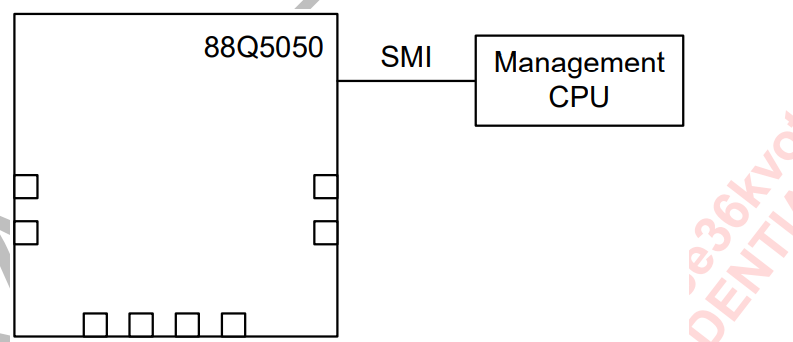
\includegraphics[scale=0.7]{pic/Snipaste_2021-10-23_19-03-03.png}
    \caption{SMI 接口管理 Switch}
    \label{fig:smi_interface}
\end{figure}

\begin{figure}[ht]
    \centering
    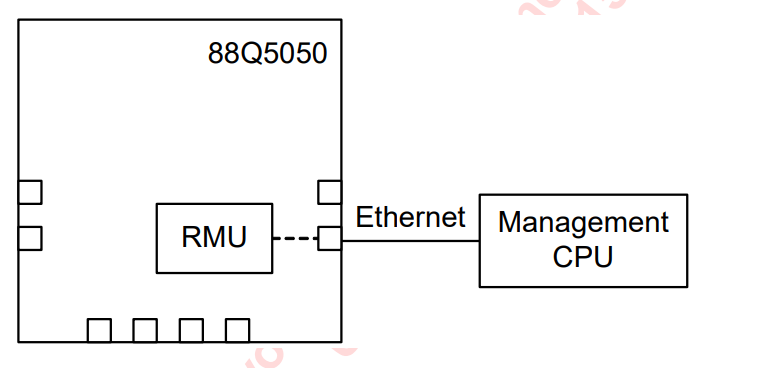
\includegraphics[scale=0.7]{pic/Snipaste_2021-10-23_19-04-54.png}
    \caption{以太网接口管理 Switch}
    \label{fig:eth_interface}
\end{figure}

\section{Swtich 核心}
\subsection{功能描述} 
本节对 Switch 所有端口一致的功能进行描述。Switch 核心的功能分为以下几个部分:

\begin{itemize}
    \item Switch 基础功能:所有帧操作模式通用的功能。
    \item 普通网络帧模式:IEEE 标准下未打 tag 帧和打 tag 帧,或自定义 Swtich 端口且至少有一个 \textbf{Provider} 端口。
    \item \textbf{Provider} 帧模式: IEEE 标准 \textbf{Provider} 端口。
    \item 分布式交换机架构帧模式(Distrubuted Switch Architecture, DSA):多片 Switch 级联或连接到一个 Switch 管理 CPU。
\end{itemize}

每一个 Switch 端口可以在以下几种基础操作模式下:
\begin{itemize}
    \item 普通模式
    \item \textbf{Provider} 模式
    \item DSA 模式,包括经典模式和 EtherType
\end{itemize}

以上操作模式都通过寄存器 \lstinline{PORT offset 0x04} 的 FrameMode 字段配置。

\subsection{基础 Swtich 功能}
\subsubsection{Swtich 物理数据流向}

88Q5050接收以太网帧,并决定丢弃或从一个或多个端口发送出去。对每个以太网帧执行何种决策只是 Switch 内部任务的一种。
图\ref{fig:data_flow}显示了交换机内部的数据路径以及在帧通过 88q5050 器件时处理帧的主要功能块。每个功能块及其可配置寄存器选项在接下来的章节中描述。
本节主要关注 Switch 内部一个端口上的帧处理及策略。

\begin{figure}[ht]
    \centering
    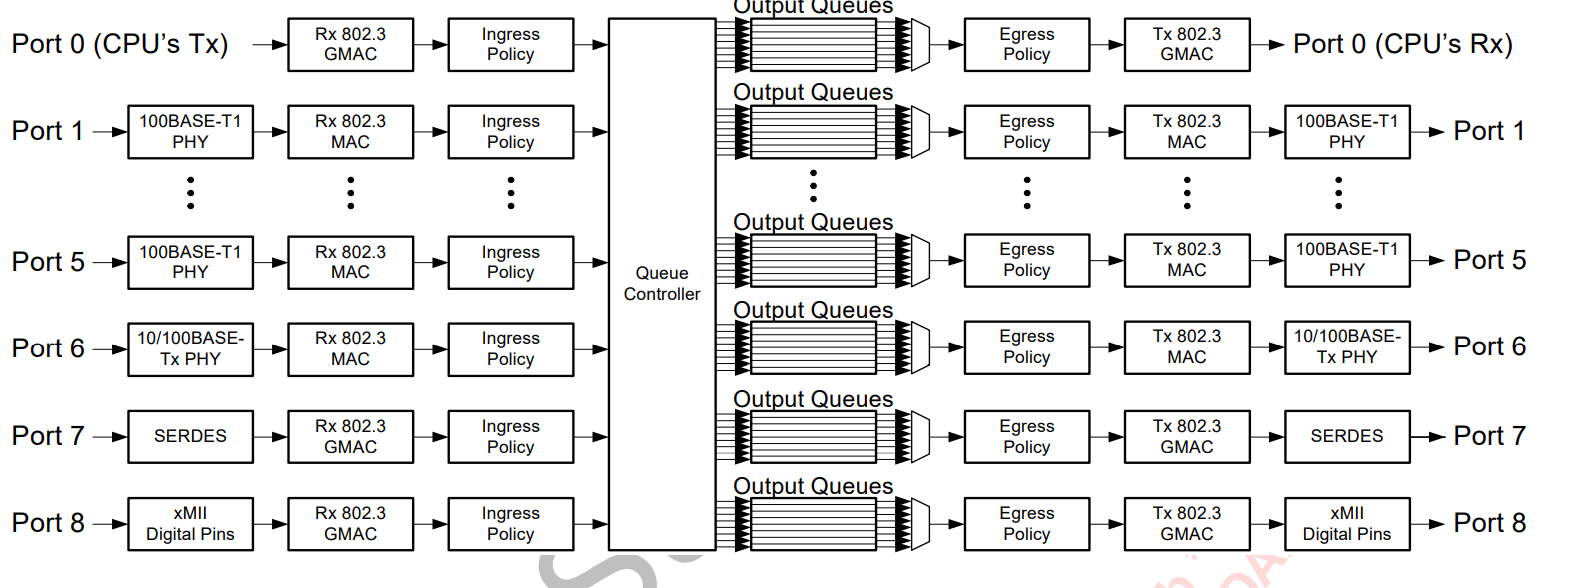
\includegraphics[scale=0.5]{pic/Snipaste_2021-10-24_16-16-48.png}
    \caption{Swtich data flow}
    \label{fig:data_flow}
\end{figure}

\subsubsection{物理接口}
每个端口都包含一个物理接口,用于从端口的 MAC 接收和传输帧。 一些端口支持多种物理接口选项,而一些仅支持部分。如果一个端口支持多个接口选项,则在同一时刻仅能使用一种。
每个端口支持的物理接口选项在\textbf{DataSheet} Device physical interfaces 章节详细描述。

\begin{note}
88q5050 的设备特点通常会和相关寄存器关联。这些寄存器按照分组组织,分别为 \lstinline{PORT},\lstinline{Global1(GLB1)},\lstinline{Global2(GLB2)} 和 \lstinline{TCAM},以及一些访问PHY的寄存器。
每一组包括 32 个 16 位寄存器,每一个端口包括这样的 32 个寄存器。组中超出 32 的特殊寄存器通过 \lstinline{offset} 引用。
如端口控制寄存器通过 \lstinline{PORT offset 0x04} 引用,因为该寄存器位于端口地址空间的 \lstinline{0x04} 地址。详细的寄存器描述可参考 寄存器手册 \textbf{Register specification}。
\end{note}

\subsubsection{介质访问控制(MAC)}
88Q5050 带有 9 个 MAC,执行 802.3 协议的所有功能,包括帧格式,帧裁剪,CRC 校验,载波侦听多路访问/冲突检测增强(CSMA/CD)和碰撞处理。
每一路 MAC 支持 10 和 100M 全双工或半双工模式,及 1G 全双工模式。连接到内部 CPU 的 MAC使用固定的 1G 速率,且只支持全双工模式。

MAC Rx 功能块检查接收到的包,并抛弃存在 CRC 错误、对齐错误和小于 64 字节的短包或大于 1522/2048/10240字节的过长包。
MAC 持续地监测它的接收线,等待前导段字节及其后的帧起始段。接下来的 6 个字节用于包的目的 mac 地址,再接下来的 6 个字节为包的源地址。
这两个地址是 Switch 功能操作的基础。接下来的 2~60个字节被检查,并可用于服务质量(QoS)或交换机做出的策略决定。
最后的 4 个字节是包的帧校验序列(FCS)。FCS 必须满足 IEEE 802.3 CRC32 需求,负责该包会被丢弃。具体格式见图\ref{fig:eth_mac_format}。

\begin{figure}[ht]
    \centering
    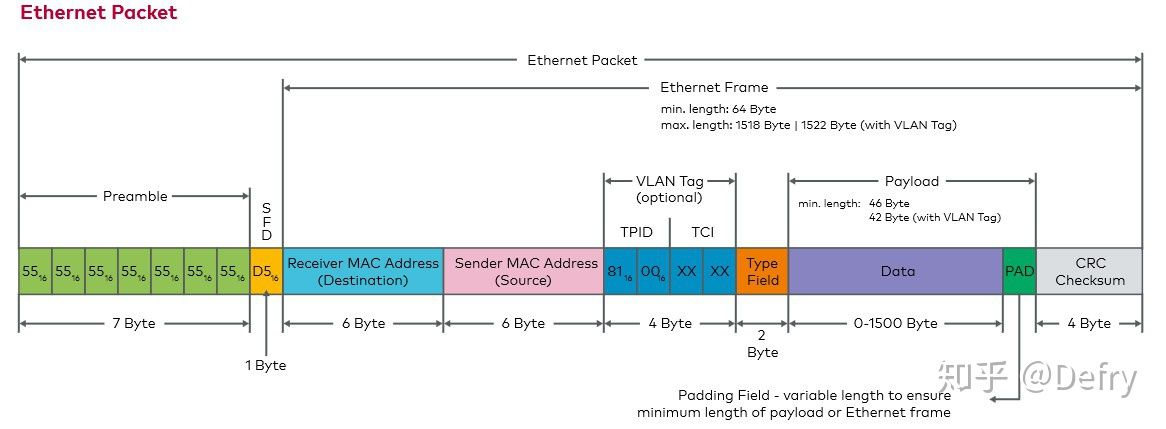
\includegraphics[scale=0.5]{pic/eth_mac_format.jpg}
    \caption{Ethernet mac frame format}
    \label{fig:eth_mac_format}
\end{figure}

在一个包被发送之前,发送功能块会检查发送线是否可用于发送。当端口为全双工模式时,发送线总是处于可用,但是在半双工模式下,可能处于不可发送状态。
一旦发送线时忙碌状态,发送推迟发送,并进行等待。当发送线可用时,发送器确保在发送帧前的 56 位前导码和 8 位 SFD 之前出现至少 96 位的最小包间隙。
实际的帧在 SFD 后立即发送。

在半双工模式下, 88q5050 在发送时监测碰撞信号。如果监测到碰撞(PHY同时在发送和接收数据)。MAC 发送一个拥挤信号(Jam pattern),然后延迟重传一段随机时间,该时间由 IEEE 802.3 
回退算法决定(backoff algorithm)。在全双工模式下则忽略碰撞和回退算法。

\subsubsection{统计计数器}
TODO

\subsubsection{调试计数器}
TODO

\subsection{基础 Switch 操作}
Switch 的首要任务是处理帧,涉及到以下功能块:
\begin{itemize}
    \item 入口规则
    \item 队列控制
    \item 输出队列
    \item 出口规则
\end{itemize}

通过交换机的正常数据包流和处理涉及学习如何将数据包交换到正确的 MAC 且仅交换到唯一的 MAC。Switch 通过记录每个包的源地址,学习端点连接了哪一个端口。
一旦 mac 地址和端口的映射关系学习到后,所有后续的包都根据目的 mac 地址发送到学习到端口。如果一个包定向到一个新的,当前没有学到的目的 mac 地址,该包将被发送到所有的端口,当然除了接收到该包的端口。
这保证了包从正确的端口接收,并且当目的端口有响应后,它的地址将被学习,并用于后续包的传输。

受物理存储的限制,Switch 仅学习 MAC 地址映射的一个小的子集。Switch 仅学习当前激活的 MAC 地址。当端口设备移动到另一个端口后,新的 MAC 地址和端口的映射关系必须重新学习,旧的映射关系应当被替换掉。
这些相关的议题在以下章节 Aging 和 Station move handing 讨论。基础的,MAC 地址和端口的映射关系仅能有效一段时间,一般为 5 分钟。

接下来章节讨论 88q5050 如何执行基础功能。

\subsubsection{查表引擎}
88q5050 查表引擎或地址解析单元使用每一个接收帧的 DA, SA 及 VID 字段。以很快的速度执行地址搜索、地址学习和地址老化功能。
可以在更短的时间内为所有端口执行 DA 和 SA 查找功能,然后在每个端口上接收 64 字节帧。

地址数据库使用哈希技术用于快速存储和检索。将 48 位地址哈希为更少位数的结果,将有可能一些 MAC 地址有相同的哈希地址。这称为哈希碰撞,该问题通过对每个哈希地址添加 4 个 \textbf{bins}(?)解决。
这样对于每个哈希值,最多可存储 4 个 MAC地址。这使得地址数据库在存储相同数量的随机 MAC 地址时,可以更小。

地址数据库存储在嵌入式 SRAM 中,大小为 1024 个条目,默认的老化时间为 5 分钟。老化时间可以以 3.75s 的时间递增,范围为 0s(禁止老化) 至 16 分钟。
该配置可通过 ATC 控制寄存器 \lstinline{GLB1 offset 0x0A}修改。

\subsubsection{地址搜索或翻译}
地址搜索引擎用于在地址数据库中查找地址,以获取输出的一个或多个端口。如果是多个端口,则该帧被泛洪到响应端口。
输出端口的列表称为目标端口向量表(DPV)。搜索引擎仲裁来自端口的目标地址查找请求,并一次授予一个查找权限。
查找地址首先被哈希处理,然后从地址数据库中读取数据,查找 MAC 地址。对于一个哈希位置,可以最多存储 4 个 MAC 地址。

\begin{itemize}
    \item 如果找到一个匹配的 MAC 地址,ATU 返回 DPV 给入口规则块,在这一步中 DPV 可能在包被发送到输出端口前被修改。如果查找到条目中包含链路聚合 ID,则 LAG ID 被
转换为使用 LAG 映射表的 DPV(LAG 映射表在 \lstinline{GLB2 offset 0x08} 寄存器配置)。
    \item 如果没有匹配到 MAC 地址,则入口规则块为所有的输入端口使用默认的 DPV,典型行为为泛洪帧给所有端口。
\end{itemize}

如果帧的目的地址是多播地址\footnote{多播地址不能自动学习,必须通过 CPU 或 EEPROM 方式手从载入}或广播地址,则该地址的搜索方法和单播地址的处理方式相同,帧的处理方式也类似。该特征被用于多播地址过滤。
88q5050 支持多个分离的地址数据库,搜索方式通过端口默认转发信息数据库(FID, FID[3:0] \lstinline{PORT offset 0x06},FID[7:4] \lstinline{PORT offset 0x05})控制,或 VTU 根据入口期间分配给帧的 VID 分配给帧的 FID 。

\begin{figure}[ht]
    \centering
    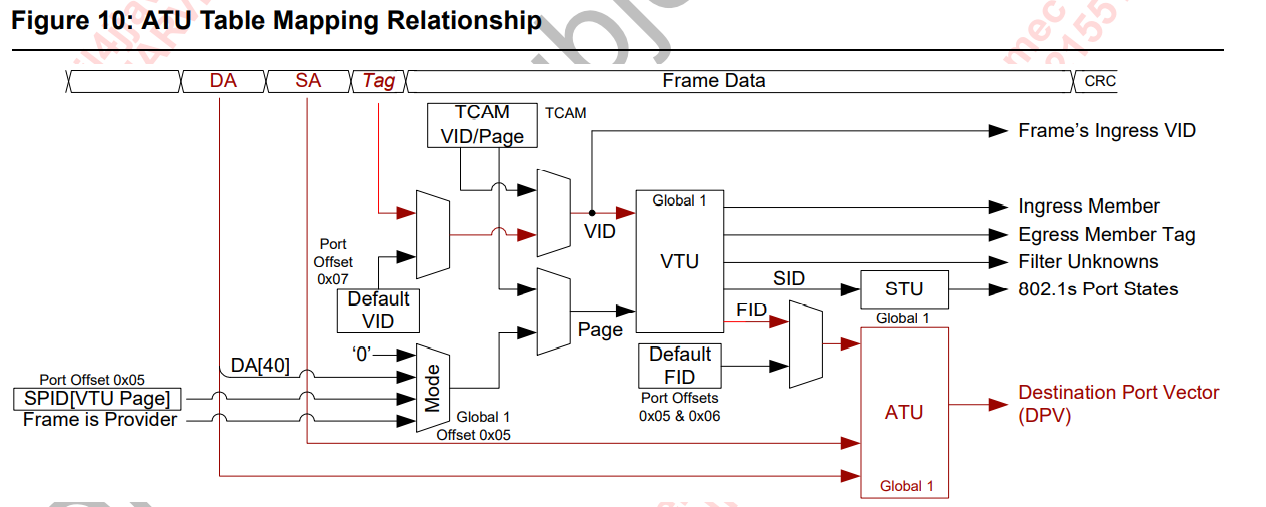
\includegraphics[scale=0.7]{pic/Snipaste_2021-10-25_15-05-41.png}
    \caption{ATU table 映射关系}
    \label{fig:atu_table_mapping}
\end{figure}

\subsubsection{自动地址学习}
地址学习引擎用于学习入口帧的源地址。最多可存储 1024 条地址和端口的映射关系条目。当从地址数据库中找不到源地址时,ATU 进入学习模式,将新的地址端口映射关系存储到数据库中,并刷新老化时间。
如果已经找到源地址,则端口信息和老化时间进行更新。当端口外接设备被移除时,端口编号和 LAG ID 被更新或纠正。只要 MAC 地址处于激活状态,条目的老化时间就一直被更新。这确保了条目不会被过早的移除。

当新地址被添加到数据库后,将被哈希化,并存储到对应哈希位置的前四个位置中。如果四个位置全满,则通过查看每个现有条目的老化时间来替换最近最少使用条目的算法进行解决(最老的,EntryState)。
如果四个条目的老化时间相同,则使用第一个位置。如果四个地址都是静态的,则不会学习到地址,且将会产生一个 ATU 问题中断\lstinline{GLB1 offset 0x00}。
如果源端口不是一个LAG端口\footnote{寄存器\lstinline{PORT offset 0x05} 的 LAGPort bit 为 0},端口信息和地址映射存储在端口关联向量表(PAV,\lstinline{PORT offset 0x0B})中。

88q5050 通过 FID 支持多个分离的地址数据库。如果使用不同的 FID 值,FID 允许使用不同的端口映射多次学习到的相同 mac 地址。

\begin{itemize}
    \item 如果 802.1q 被禁止,则端口的 FID 决定 MAC 地址添加到哪一个地址数据库。
    \item 如果使能 802.1q,帧VLAN ID(VID)关联的 FID 决定了存储 MAC 地址的地址数据库,前提是VLAN数据库中包含帧的 VLAN ID。如果 VLAN 数据库中不包含VID,则使用端口的 FID 替换。
\end{itemize}

通过清零端口的 PAV(\lstinline{PORT offset 0x0B}), 端口的自学习功能可以被单独禁止。当端口的状态(PortState \lstinline{PORT offset 0x04})是 disabled 或 blocking/listening 时,自学习也关闭。

对于 Switch 管理帧,不进行自学习。包含 pause frame, bridge protocal data unit(BPDU), LAC 和其他管理帧。\textcolor{red}{\textbf{除了Forward类型的 DSA 标记帧之外的 DSA 标记帧也被视为管理帧}}。

\subsubsection{硬件地址学习限制}
TODO

主要是对硬件自动学习映射关系的条目数进行限制,该功能可使能,也可禁止。

\subsubsection{自动地址老化}
地址老化用于确保如果一个节点从网络中移除后,或不在处于激活状态,与之相关的条目将在一定时间内从地址数据库中移除。
老化可以给新的激活的的地址提供空间。老化的时间可以通过编程方式进行配置,如相关寄存器的 AgeTime 字段(\lstinline{GLB1 offset 0x0A})中。

除非 AgeTime 字段为 0,则芯片持续运行地址老化处理。通过周期性的扫描地址数据库已实现老化处理。每次扫描地址数据库,ATU 读取每一条有效条目并更新老化时间,递减时间通过 EntryState 字段定义。
当 EntryState 为 0 时,条目认为是无效的,并从数据库中清除。如果 HoldAt1 字段(\lstinline{PORT offset 0x0B})置位,则当EntryState 为 1 时,不在继续递减。

新的或刚更新的单播 MAC 地址的 EntryState 值为 0x7。一个清除的或无效的条目状态值为 0x0。0x1 至 0x6 表示单播地址的老化程度,其中 0x1 代表最老化。
该方式将老化程度分为 7 类,在需要地址替换时更为精确。

\subsubsection{CPU 直接地址学习和移除}
通过 CPU 直接学习 MAC地址和端口映射关系。

TODO

\subsubsection{802.1X 源 MAC 地址检查}
TODO

\subsubsection{多地址数据库支持(FID)}
Swtich 芯片 ATU 支持多达 256 个分离且独立的地址数据库。多地址数据库用于通过 vlan 或端口隔离 mac 地址,因此相同的 mac 地址可以在具有不同端口映射的地址数据库中多次出现。
芯片使用 802.1Q中定义的 FID 机理来隔离地址数据库。虽然地址数据库是通过fid值隔离的,但它并没有被fid值分成相等的段。
每个数据库的数量可以为一个也没有到所有可能的 mac 地址或任何数量的值。从 1 到 256 的 FID 值可以被使用。每一个 FID 只使用它需要的 mac 地址条目,并为所有其他数据库留下所有剩余的 ATU 条地址和端口的映射关系条目。当从地址数据库中找不到源地址时,ATU 

当一帧报文从端口进入后就分配了 FID。帧 FID 和帧的源地址及目的地址一起发送给 ATU,已进行 mac 地址的查找或学习。FID 值通过以下优先级方式确定:
\begin{itemize}
    \item FID 和 VTU 中的 VID 值相关。这需要 VTU 中帧的 VID值有效。
    \item FID 和对应输入端口的寄存器值有关(FID, FID[3:0] \lstinline{PORT offset 0x06},FID[7:4] \lstinline{PORT offset 0x05})
\end{itemize}

如果不使用多个地址数据库,则所有 FID 寄存器值保持复位值 0x0(\lstinline{PORT offset 0x5 0x06, GLB1 offset 0x01 0x02})。

帧的 FID 通常通过 VID值确定。多个 VID值可以映射到一个 FID,以共享 VLAN 地址数据库。

\section{普通网络端口}
普通网络模式可以通过设置寄存器字段 FrameMode 为0 开启(\lstinline{PORT offset 0x04})中。

\subsection{入口规则}
入口规则块用于修改正常的数据包流,以限制哪些帧被允许进入Switch。所有端口具有相同的入口规则处理能力,具体如下:

\begin{itemize}
    \item 非 MGMT 帧可以被阻止进入交换机,从而支持生成树协议
    \item 帧源 mac 地址可以授权,帧可能被丢弃或映射到内部 cpu,以支持 802.1X。
    \item 
\end{itemize}

\section{Provider mode 端口}

\section{DSA 端口}

% \input{ch1/section2}
% \input{ch1/section3}
% \input{ch1/section4}
% \input{ch1/section5}
% \input{ch1/section6}
% \input{ch1/section7}
% \input{ch1/section8}
	\chapter{存储配置}
\section{CAN}
% \input{ch1/section2}
% \input{ch1/section3}
% \input{ch1/section4}
% \input{ch1/section5}
% \input{ch1/section6}
% \input{ch1/section7}
% \input{ch1/section8}
	\chapter{诊断配置}
\section{CAN}

	\chapter{通信配置}
\section{CAN}

	\chapter{网络管理配置}
\section{CAN}

    \chapter{数据结构与算法}
\section{前导零与后导零计算}

前导零:即一个数的二进制,从 MSB 开始数,直到遇到第一个1,前面几有个零。如 \lstinline{0x00FFFFFF} 前导零为8; \lstinline{0xF0000000} 前导零为0; \lstinline{0x08010002} 前导零为4。

后导零则与之相反,从 LSB 开始计算。两种情况下,具体的代码实现见后两节。

\subsection{前导零}

此代码从 UCOS 实现源码中截取,详见博客\cite{65TiaoXiaoXiJiSuanQianDaoLingCYuYanShiXianU013073067DeBoKeCSDNBoKe}。
\lstinputlisting[
    style       =   C,
    language = C,
    caption     =   {前导零计算},
]{ch7/lead_zero.c}

\subsection{后导零}

\lstinputlisting[
    style       =   C,
    language = C,
    caption     =   {后导零计算},
]{ch7/back_zero.c}

\section{二进制数位翻转}

\begin{lstlisting}[language=C,style=C]
uint16 eth_bitReverse(uint16 value)
{
    value = (((value & 0xaaaa) >> 1) | ((value & 0x5555) << 1));
    value = (((value & 0xcccc) >> 2) | ((value & 0x3333) << 2));
    value = (((value & 0xf0f0) >> 4) | ((value & 0x0f0f) << 4));
    value = (((value & 0xff00) >> 8) | ((value & 0x00ff) << 8));

    return(value);
}
\end{lstlisting}


	\nocite{*} 
	\printbibliography
\end{document}